%% 
%% Copyright 2007, 2008, 2009 Elsevier Ltd
%% 
%% This file is part of the 'Elsarticle Bundle'.
%% ---------------------------------------------
%% 
%% It may be distributed under the conditions of the LaTeX Project Public
%% License, either version 1.2 of this license or (at your option) any
%% later version.  The latest version of this license is in
%%    http://www.latex-project.org/lppl.txt
%% and version 1.2 or later is part of all distributions of LaTeX
%% version 1999/12/01 or later.
%% 
%% The list of all files belonging to the 'Elsarticle Bundle' is
%% given in the file `manifest.txt'.
%% 

%% Template article for Elsevier's document class `elsarticle'
%% with numbered style bibliographic references
%% SP 2008/03/01

%%\documentclass[preprint,12pt]{elsarticle}

%% Use the option review to obtain double line spacing
%% \documentclass[authoryear,preprint,review,12pt]{elsarticle}

%% Use the options 1p,twocolumn; 3p; 3p,twocolumn; 5p; or 5p,twocolumn
%% for a journal layout:
%% \documentclass[final,1p,times]{elsarticle}
%% \documentclass[final,1p,times,twocolumn]{elsarticle}
\documentclass[final,3p,times]{elsarticle}
%% \documentclass[final,3p,times,twocolumn]{elsarticle}
%% \documentclass[final,5p,times]{elsarticle}
%% \documentclass[final,5p,times,twocolumn]{elsarticle}

%% For including figures, graphicx.sty has been loaded in
%% elsarticle.cls. If you prefer to use the old commands
%% please give \usepackage{epsfig}

%% The amssymb package provides various useful mathematical symbols
\usepackage{amssymb}
%% The amsthm package provides extended theorem environments
%% \usepackage{amsthm}

%% The lineno packages adds line numbers. Start line numbering with
%% \begin{linenumbers}, end it with \end{linenumbers}. Or switch it on
%% for the whole article with \linenumbers.
%% \usepackage{lineno}

\usepackage{latexsym}
\usepackage[latin1]{inputenc}
\usepackage{times}
\usepackage[english]{babel}
\usepackage{amssymb}
\usepackage{algorithm}
\usepackage{algorithmic}
\usepackage{epsfig,shadow,amssymb,bm}

\usepackage{graphicx}
\usepackage{tikz}
\usetikzlibrary{shapes,arrows}
\usetikzlibrary{positioning}
\usetikzlibrary{arrows,automata,decorations,shapes}
\tikzset{
  treenode/.style = {shape=rectangle, rounded corners,
                     draw, align=center,
                     top color=white, bottom color=blue!20},
  root/.style     = {treenode, font=\Large, bottom color=red!30},
  env/.style      = {treenode, font=\ttfamily\normalsize},
  dummy/.style    = {circle,draw}
}

\journal{}

%%%%%%%%%%%%%%%%%%%%%%%%%%%%%%%%%%%%%%%%%%%%%%%%%%%%%%%%%%%%%%%%%%%%%
%% Place any additional macros here.  Please use \newcommand* where
%% possible, and avoid layout-changing macros (which are not used
%% when typesetting).
%%%%%%%%%%%%%%%%%%%%%%%%%%%%%%%%%%%%%%%%%%%%%%%%%%%%%%%%%%%%%%%%%%%%%
\newcommand*\mycommand[1]{\texttt{\emph{#1}}}

%%%%%%%%%%%%%%%%%%%%%%%%%%%%%%%%%%%%%%%%%%%%%%%%%%%%%%%%%%%%%%%%%
%% The following definitions are to extend the LaTeX algorithmic
%% package with SWITCH statements and one-line structures.
%% The extension is by
%%   Prof. Farn Wang
%%   Dept. of Electrical Engineering,
%%   National Taiwan University.
%%
\newcommand{\SWITCH}[1]{\STATE \textbf{switch} (#1)}
\newcommand{\ENDSWITCH}{\STATE \textbf{end switch}}
\newcommand{\CASE}[1]{\STATE \textbf{case} #1\textbf{:} \begin{ALC@g}}
\newcommand{\ENDCASE}{\end{ALC@g}}
\newcommand{\CASELINE}[1]{\STATE \textbf{case} #1\textbf{:} }
\newcommand{\DEFAULT}{\STATE \textbf{default:} \begin{ALC@g}}
\newcommand{\ENDDEFAULT}{\end{ALC@g}}
\newcommand{\DEFAULTLINE}[1]{\STATE \textbf{default:} }
%%
%% End of the LaTeX algorithmic package extension.
%%%%%%%%%%%%%%%%%%%%%%%%%%%%%%%%%%%%%%%%%%%%%%%%%%%%%%%%%%%%%%%%%

\begin{document}



%% Title, authors and addresses

%% use the tnoteref command within \title for footnotes;
%% use the tnotetext command for theassociated footnote;
%% use the fnref command within \author or \address for footnotes;
%% use the fntext command for theassociated footnote;
%% use the corref command within \author for corresponding author footnotes;
%% use the cortext command for theassociated footnote;
%% use the ead command for the email address,
%% and the form \ead[url] for the home page:
%% \title{Title\tnoteref{label1}}
%% \tnotetext[label1]{}
%% \author{Name\corref{cor1}\fnref{label2}}
%% \ead{email address}
%% \ead[url]{home page}
%% \fntext[label2]{}
%% \cortext[cor1]{}
%% \address{Address\fnref{label3}}
%% \fntext[label3]{}



\title{Weka for Feature Selection and Its Application for Energy Efficiency in Smart Buildings}

%% use optional labels to link authors explicitly to addresses:
%% \author[label1,label2]{}
%% \address[label1]{}
%% \address[label2]{}









%% \linenumbers

%% main text


\section{Background}
\label{sec:background}

\subsection{Feature Selection}

{\em Feature Selection} (FS) is defined in~\cite{Liu:1998:FSK:551944} as the process of eliminating features from the data base that are irrelevant to the task to be performed. 
FS facilitates data understanding, reduces the measurement and storage requirements, reduces the computational process time, and reduces the size of a data set, 
so that model learning becomes an easier process. 
An FS method is basically a \textit{search strategy} where the performance of candidate subsets is measured with a given  \textit{evaluator}. The search space for
candidate subsets has cardinality $O(2^w)$, where $w$ is the number of features. A \textit{stopping criterion} establishes when the feature
selection process must finish. It can be defined as a control procedure
that ensures that no further addition or deletion of features does
produce a better subset, or it can be as simple as a counter of iterations. FS methods are typically categorized into \textit{wrapper\textit{}}, \textit{filter} and \textit{embedded}, \textit{univariate} and \textit{multivariate} methods. \textit{Wrapper methods} \cite{kohavi1997wrappers} use a predetermined learning algorithm to determine the quality of selected features according to an evaluation metric \cite{Japkowicz:2011:ELA:1964882}. \textit{Filter methods} apply statistical measures to evaluate the set of attributes \cite{Kar10, Hal98, Ami05}. \textit{Embedded methods} achieve model fitting and feature selection simultaneously \cite{Sal94}. \textit{Multivariate methods} evaluate features in batches. \textit{Univariate methods} evaluate each feature independently.




\subsection{Feature Selection in Weka}

In the \textit{Waikato Environment for Knowledge Analysis} (\textit{Weka}) \cite{Weka}, FS is implemented with the  \textit{weka.attribute\-Selection.\-AttributeSelection} class of the \textit{weka.attributeSelection} package through two components: the \textit{search strategy} (\textit{weka.\-attributeSelection.ASSearch} abstract class) and the \textit{evaluator} (\textit{weka.attributeSelection.ASEvaluation} abstract class). This allows users and programmers to configure a multitude of different methods for FS, both filter and wrapper, univariate and multivariate. Evaluators with names ending in \textit{SubsetEval} configure multivariate methods, whereas those with names ending in \textit{AttributeEval} configure univariate methods.  For multivariate wrapper FS methods, the \textit{weka.attributeSelection} package has the \textit{weka.attributeSelection.WrapperSubsetEval}  class which evaluates attribute sets by using a learning scheme with  cross-validation and a performance measure. For univariate wrapper FS methods, the \textit{weka.attributeSelection.Classi\-fierAttributeEval} class evaluates the worth of an attribute by using a user-specified classifier, cross-validation and a performance evaluation measure to use for selecting attributes. Since the FS and classification processes must be executed in bach mode, Weka offers the class \textit{weka.classifiers.meta.AttributeSelected\-Classifier} which is a meta-classifier where dimensionality of data is reduced by attribute selection before being passed on to a learning algorithm.

\section{Experiments and results}

\begin{figure}[h!]
	
	\begin{center}
		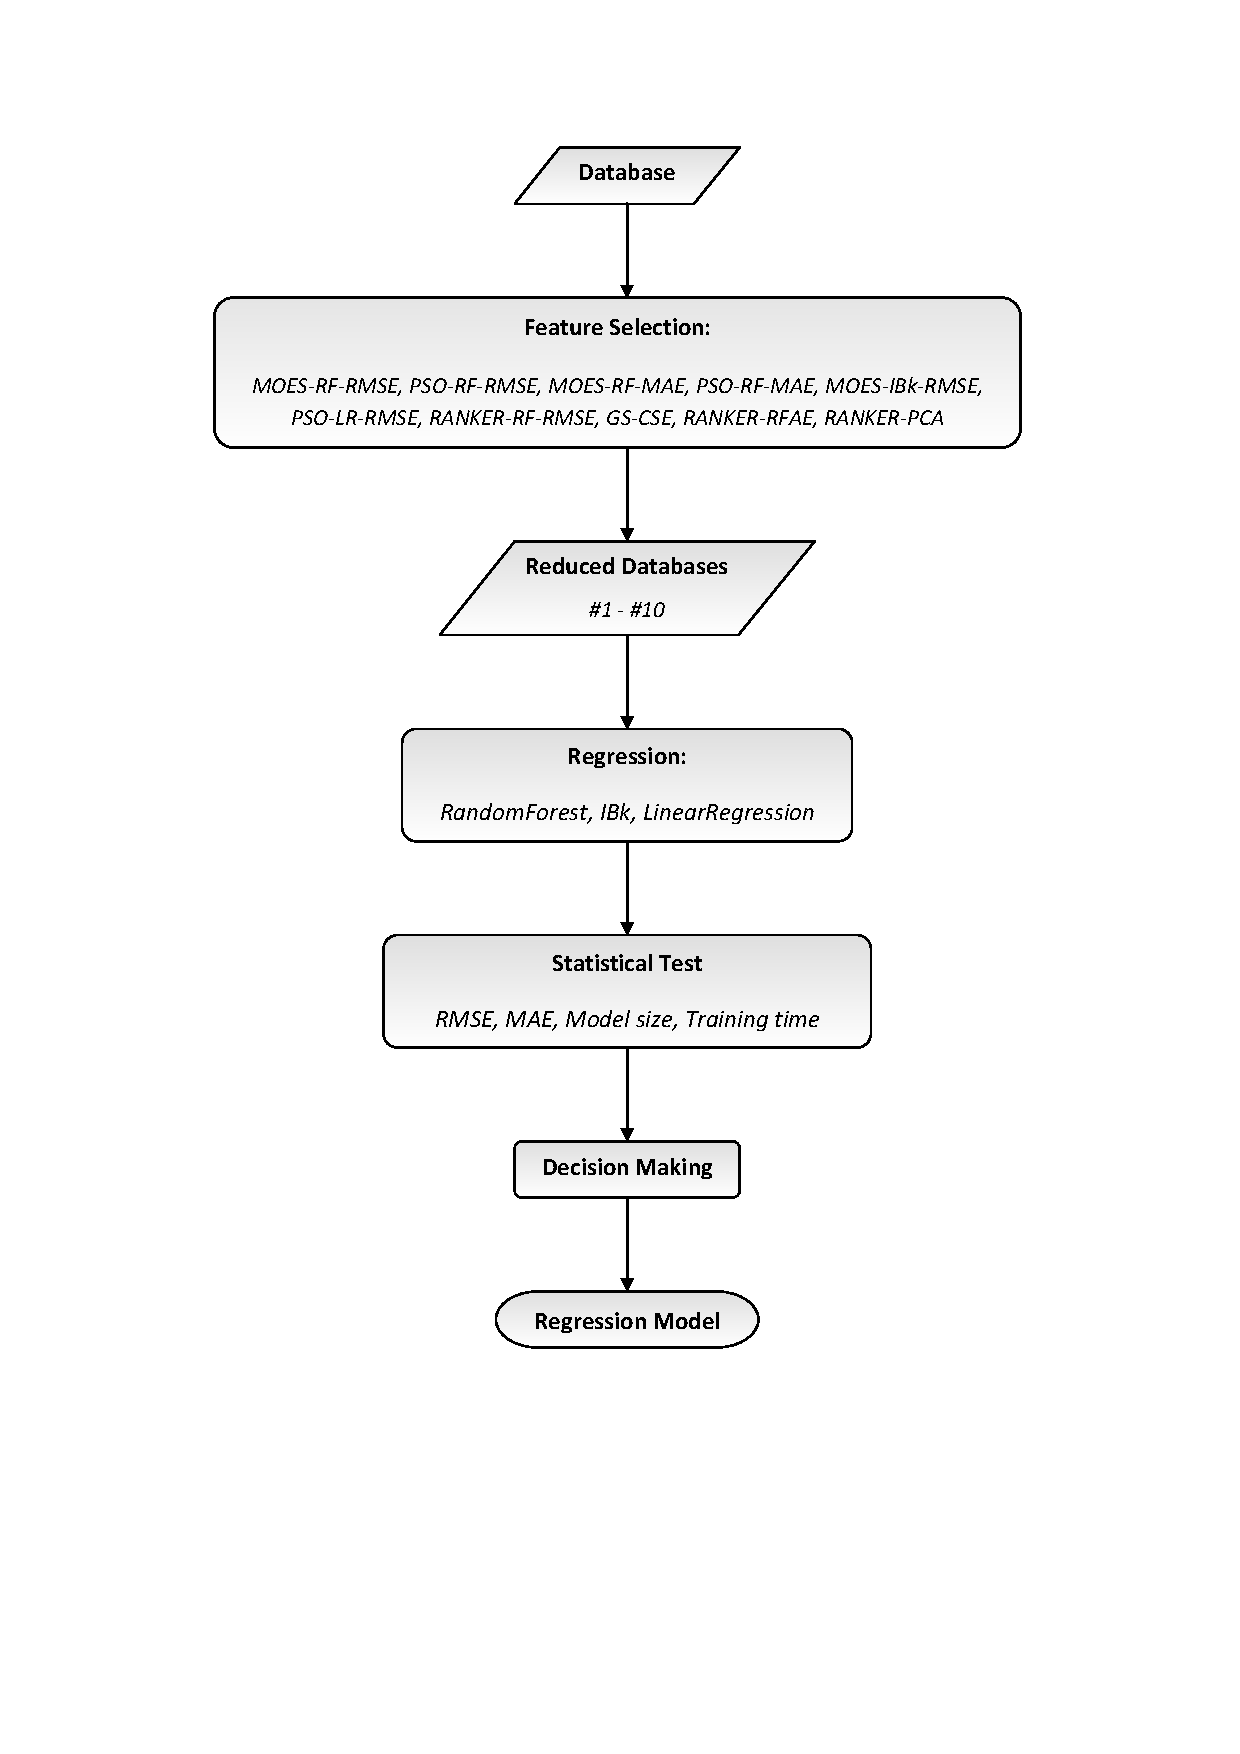
\includegraphics[scale=0.55]{metodology.pdf}
		\vskip -3cm
		\caption{Metodology for Feature Selection for regression.}
		\label{fig:grafico-metod} 
	\end{center}
\end{figure}

We have followed the methodology shown in the Figure \ref{fig:grafico-metod} to perform FS. We have systematically applied 10 different FS methods for regression shown in Table \ref{FSM} and graphically in Figure \ref{fig:FSmethods}. In Table \ref{FSM}, \textit{Database \#Id} denotes the identifier of the reduced database generated with each FS method. Each FS method is the result of a specific choice among the search strategy, the evaluator, and the performance metric (for wrapper FS methods). We considered for this research seven wrapper FS methods and three filter FS methods. Among them, seven FS methods are multivariate and three FS methods are univariate. Table \ref{PFSM} shows the parameters used for each FS method.




\begin{table}[h]
	\begin{center}
		\footnotesize{\begin{tabular}{ccccc}\hline
	\textit{\textbf{Database \#Id.}} & \textit{\textbf{FS method}} & \textit{\textbf{Name}} & \textit{\textbf{Search strategy}} & \textit{\textbf{Evaluator}} \\\hline
	
	\textit{\#1} & Wrapper Multivariate & \textit{MOES-RF-RMSE} & \textit{MultiObjectiveEvolutionarySearch} & \textit{RandonForest (RMSE)}  \\
	\textit{\#2} &  Wrapper Multivariate & \textit{PSO-RF-RMSE} & \textit{PSOSearch} & \textit{RandonForest (RMSE)}  \\
	\textit{\#3} & Wrapper Multivariate & \textit{MOES-RF-MAE} & \textit{MultiObjectiveEvolutionarySearch} & \textit{RandonForest (MAE)}  \\	

	\textit{\#4} & Wrapper Multivariate & \textit{PSO-RF-MAE} & \textit{PSOSearch} & \textit{RandonForest (MAE)}  \\
	\textit{\#5} & Wrapper Multivariate & \textit{MOES-IBk-RMSE} & \textit{MultiObjectiveEvolutionarySearch} & \textit{IBk (RMSE)}  \\	
	\textit{\#6} & Wrapper Multivariate & \textit{PSO-LR-RMSE} & \textit{PSOSearch} & \textit{LinearRegression (RMSE)}  \\
	\textit{\#7} &  Wrapper Univariate & \textit{RANKER-RF-RMSE} & \textit{Ranker} & \textit{RandonForest (RMSE)}  \\
	\textit{\#8} &  Filter Multivariate & \textit{GS-CSE} & \textit{GreedyStepwise} & \textit{ConsistencySubsetEval}  \\
	\textit{\#9} &  Filter Univariate & \textit{RANKER-RFAE} & \textit{Ranker} & \textit{ReliefFAttributeEval}  \\
	\textit{\#10} &  Filter Univariate & \textit{RANKER-PCA} & \textit{Ranker} & \textit{PrincipalComponents}  \\
   \hline		
	\end{tabular}}
	\end{center}
	\caption{Proposed Feature Selection methods for regression.}
	\label{FSM}
\end{table}

\begin{table}[h!]
	\begin{center}
		\footnotesize{\begin{tabular}{cc}\hline
			\textit{\textbf{Database \#Id.}} & \textit{\textbf{Parameters}} \\\hline
			
			\textit{\#1} &  -E ``weka.attributeSelection.WrapperSubsetEval \\
			& -B weka.classifiers.trees.RandomForest  -F 5 -T 0.01 -R 1 \\
			& -E DEFAULT -- -P 100 -I 10 -num-slots 1 -K 0 -M 1.0 -V 0.001 -S 1" \\
			& -S ``weka.attributeSelection.MultiObjectiveEvolutionarySearch \\ 
			& -generations 1000 -population-size 100 -seed 1 -a 0 "\\
			
			
			\textit{\#2} &  -E ``weka.attributeSelection.WrapperSubsetEval \\
			& -B weka.classifiers.trees.RandomForest -F 5 -T 0.01 -R 1 \\
			& -E DEFAULT -- -P 100 -I 10 -num-slots 1 -K 0 -M 1.0 -V 0.001 -S 1" \\
			& -S ``weka.attributeSelection.PSOSearch -N 20 -I 1000 -T 0 \\
			&  -M 0.01 -A 0.33 -B 0.33 -C 0.34  -S 1"\\
			
			\textit{\#3} &  -E ``weka.attributeSelection.WrapperSubsetEval \\
			& -B weka.classifiers.trees.RandomForest  -F 5 -T 0.01 -R 1 \\
			& -E MAE -- -P 100 -I 10 -num-slots 1 -K 0 -M 1.0 -V 0.001 -S 1" \\
			& -S ``weka.attributeSelection.MultiObjectiveEvolutionarySearch \\ 
			& -generations 1000 -population-size 100 -seed 1 -a 0 "\\
			
			
			\textit{\#4} &  -E ``weka.attributeSelection.WrapperSubsetEval \\
			& -B weka.classifiers.trees.RandomForest -F 5 -T 0.01 -R 1 \\
			& -E MAE -- -P 100 -I 10 -num-slots 1 -K 0 -M 1.0 -V 0.001 -S 1" \\
			& -S ``weka.attributeSelection.PSOSearch -N 20 -I 1000 -T 0 \\
			&  -M 0.01 -A 0.33 -B 0.33 -C 0.34  -S 1"\\
			
			
			\textit{\#5} &  -E 
			 ``weka.attributeSelection.WrapperSubsetEval \\
			& -B weka.classifiers.lazy.IBk -F 5 -T 0.01 -R 1 \\
			& -E DEFAULT -- -K 1 -W 0 \\
			& -A ``weka.core.neighboursearch.LinearNNSearch \\
			& -A ``weka.core.EuclideanDistance -R first-last""  \\
			& -S ``weka.attributeSelection.MultiObjectiveEvolutionarySearch \\
			 & -generations 10 -population-size 100 -seed 1 -a 0" \\
			
			
			\textit{\#6} & -E ``weka.attributeSelection.WrapperSubsetEval \\
			& -B weka.classifiers.functions.LinearRegression -F 5 -T 0.01 -R 1 \\
			& -E DEFAULT -- -S 0 -R 1.0E-8 -num-decimal-places 4" \\
			& -S "weka.attributeSelection.PSOSearch -N 100 -I 1000 -T 0 \\
			& -M 0.01 -A 0.33 -B 0.33 -C 0.34 -R 1000 -S 1"\\
			
			
			\textit{\#7} & -E ``weka.attributeSelection.WrapperSubsetEval \\
			& -B weka.classifiers.trees.RandomForest -F 5 -T 0.01 -R 1 \\
			& -E DEFAULT -- -P 100 -I 10 -num-slots 1 -K 0 -M 1.0 -V 0.001 -S 1" \\
			& -S ``weka.attributeSelection.Ranker -T -1.8E308 -N 10"\\
			\textit{\#8} & -E ``weka.attributeSelection.CfsSubsetEval -P 1 -E 1" \\
			& -S ``weka.attributeSelection.GreedyStepwise -T -1.8E308 -N -1 -num-slots 1"\\
			\textit{\#9} & -E ``weka.attributeSelection.ReliefFAttributeEval -M -1 -D 1 -K 10" \\
			& -S "weka.attributeSelection.Ranker -T -1.8E308 -N 10"\\
			\textit{\#10} & -E ``weka.attributeSelection.PrincipalComponents -R 0.95 -A 5"\\
			& -S ``weka.attributeSelection.Ranker -T -1.8E308 -N 10"\\
			
			\hline		
		\end{tabular}}
	\end{center}
	\caption{Parameters of the Feature Selection methods for regression.}
	\label{PFSM}
\end{table}




\begin{figure}[h!]
	
	\begin{center}
		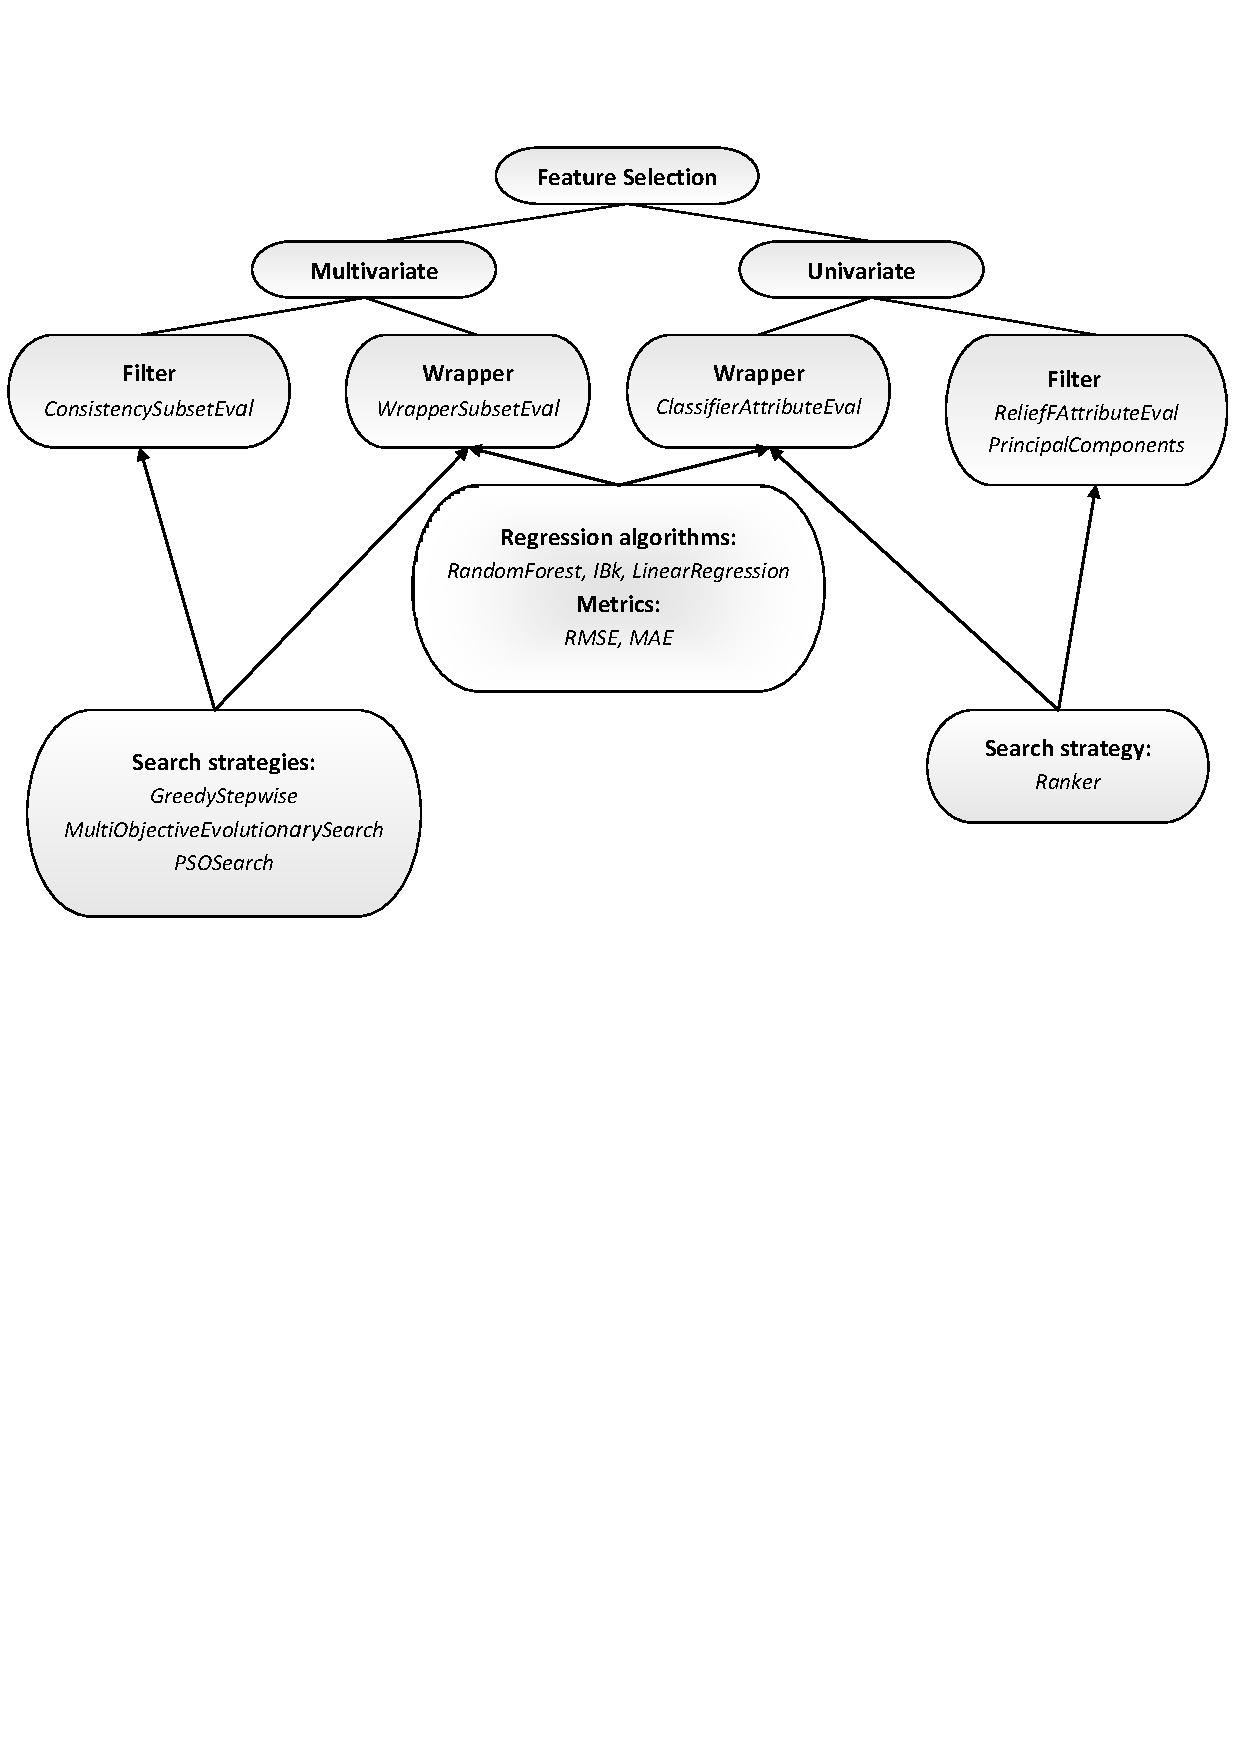
\includegraphics[scale=0.7]{FS.pdf}
		\vskip -9.5cm
		\caption{Organization chart of the proposed Feature Selection methods for regression.}\label{fig:FSmethods}
	\end{center}
\end{figure}

The following search strategies, evaluators, regression methods and performance metrics have been considered:

\begin{description}
	\item[Search strategies]
	
	For multivariate FS methods, among \textit{deterministic search strategies} we considered  \emph{GreedyStepwise}~\cite{russell2003modern}, while the employed \textit{probabilistic algorithms} are \emph{MultiObjectiveEvolutionarySearch} \cite{jimenez2016multi} and \emph{PSO\-Search} \cite{moraglio2008geometric}. \emph{GreedyStepwise} performs a greedy forward or backward search through the space of attribute subsets, stopping when the addition (forward direction) or deletion (backward direction) of any of the remaining attributes results in a decrease in evaluation, thus, it has no backtracking capability.  \textit{MultiObjectiveEvolutionarySearch}  use evolutionary computation where two objectives are optimized: the first one is chosen by the evaluator, and it is to be maximized, while the second one is the attribute subset cardinality, and it is to be minimized. The final output is given by the non-dominated solutions in the last population having the best fitness score for the first objective. \textit{PSO} optimizes a problem moving individuals (particles) around in the search-space according to the particle's position and velocity, influenced by its local best known position and the best known positions.
	
	
	For univariate FS methods, \textit{Ranker} method \cite{yujor} is required. \textit{Ranker} method ranks attributes by their individual evaluations. A threshold, or the number of attributes to retain, allows reducing the attribute set.
	
	
	
	\item[Evaluators] 
	
	We considered the  multivariate filter evaluator   \emph{ConsistencySubsetEval} \cite{liu1996probabilistic}.  \emph{ConsistencySubsetEval}  sco\-res a subset of features as a whole, by projecting the training instances according to the attribute subset, and considering the consistency of class values in the obtained instance sets. As far as univariate filter evaluators are concerned, \textit{RelieffAttributeEval} \cite{Kira:1992:PAF:141975.142034} and \textit{PrincipalComponents} \cite{WICS:WICS101}  were considered. \textit{RelieffAttributeEval} evaluates the worth of an attribute by repeatedly sampling an instance and considering the value of the given attribute for the nearest instance of the same and different class. Can operate on both discrete and continuous class data. \textit{PrincipalComponents} performs a principal components analysis and transformation of the data.  Dimensionality reduction is accomplished by choosing enough eigenvectors to account for some percentage of the variance in the original data (default 95\%). Attribute noise can be filtered by transforming to the principal components space, eliminating some of the worst eigenvectors, and then transforming back to the original space.
	
	
	
	We use the wrapper \textit{WrapperSubsetEval}  \cite{kohavi1997wrappers} for multivariate FS methods and \textit{ClassifierAttributeEval} \cite{Schaefer2016b} for univariate FS methods in conjunction with the predictors \emph{RandomForest}~\cite{breiman2001random}, \emph{IBk}~\cite{Aha:1991:ILA:104713.104717} and \textit{LinearRegression} \cite{yan2009linear}, and with the metrics \emph{root mean squared error} (\textit{RMSE}) and \textit{mean absolute error} (\textit{MAE}) \cite{Willmott200579}. {\em RandomForest} is an \emph{ensemble learning} method which constructs a forest of random trees with controlled variance, for classification or regression purposes. {\em IBk} is a simple instance-based learner that uses the class of the nearest k training instances for the class of the test instances and it is also valid for regressi�n. \textit{LinearRegression} uses the \textit{Akaike} criterion for model selection, and is able to deal with weighted instances.
	
\end{description}

Once FS was made, the next step was to perform regression with the reduced and original databases using \textit{RandomForest}, \textit{IBk} and \textit{LinearRegression}. The Table \ref{PRM} shows the parameters used for the regression methods. In order to detect over-fitting and prediction ability, the regression models have been evaluated in both full training set and 10-fold cross-validation over 10 iterations. Tables \ref{RFTS} and \ref{MFTS} show the evaluation in full training set for the \textit{RMSE} and \textit{MAE} metrics respectively. The Tables \ref{RCV}, \ref{MCV}, \ref{SMSCV} and \ref{RTCV}
show the evaluation in 10-fold cross-validation (10 iterations) for the metrics \textit{RMSE}, \textit{MAE}, \textit{Serialized\_Model\_Size} and \textit{UserCPU\_Time\_testing}\footnote{Intel (R) Core (TM) i5-4460 @ 3.20 GHz 3.20 GHz RAM 8.00 GB Operating Systems 64 bits, processor x64.} respectively. The result of the experiment has been analysed through a \textit{paired t-test (corrected)},
with 0.05 significance (being \textit{\#1\#2} 
the test base in Tables \ref{RCV} and \ref{MCV}, and \textit{RandomForest} in Tables \ref{SMSCV} and \ref{RTCV}). For each result, a mark $*$ denotes that the
result is statistically worse than the test base; similarly, a
mark $v$ denotes a statistically better result, and no mark denotes no statistically meaningful difference. Note that the reduced databases \textit{\#1} and \textit{\#2} are the same, as are the reduced databases \textit{\#3} and  \textit{\#4}, so they appear together in all the tables.

\begin{table}[h]
	\begin{center}
			\footnotesize{\begin{tabular}{cc}\hline
			\textit{\textbf{Name}} & \textit{\textbf{Parameters}} \\\hline
			
			\textit{RandomForest} & -P 100 -I 500 -num-slots 1 -K 0 -M 1.0 -V 0.001 -S 1\\
			\textit{IBk} & weka.classifiers.lazy.IBk -K 1 -W 0 \\
			& -A ``weka.core.neighboursearch.LinearNNSearch \\
			& -A ``weka.core.EuclideanDistance -R first-last""\\
			\textit{LinearRegression} & -S 0 -R 1.0E-8 -num-decimal-places 4\\\hline		
		\end{tabular}}
	\end{center}
	\caption{Parameters of the regression methods.}
	\label{PRM}
\end{table}	

\begin{table}[h]
	\begin{center}
			\footnotesize{\begin{tabular}{cccc}\hline
			\textit{\textbf{Database \#Id.}} & \textit{\textbf{RandomForest}} & \textit{\textbf{IBk}} & \textit{\textbf{LinearRegression
					}} \\\hline
			
		\textit{\#1\#2} & 4.2267 & 0.0 & 66.8625 \\	
		\textit{\#3\#4} & 4.2734 & 15.8069 & 66.8642 \\	
		\textit{\#5} & 4.6102 & 0.0 & 69.5321 \\
		\textit{\#6} & 9.3867 & 0.0 &  54.7665\\
		\textit{\#7} & 5.8233 & 0.0 & 62.1653\\
		\textit{\#8} & 6.8531 & 0.0 & 56.583 \\
		\textit{\#9} & 10.9122 & 7.0239 & 56.5407\\
		\textit{\#10} & 16.6868 & 0.0 & 58.8544\\
		\textit{Original} & 10.0615 & 0.0 & 54.6545\\
			\hline		
		\end{tabular}}
	\end{center}
	\caption{\textit{RMSE} with full training set.}
	\label{RFTS}
\end{table}

\begin{table}[h]
	\begin{center}
			\footnotesize{\begin{tabular}{cccc}\hline
			\textit{\textbf{Database \#Id.}} & \textit{\textbf{RandomForest}} & \textit{\textbf{IBk}} & \textit{\textbf{LinearRegression
				}} \\\hline
				
				\textit{\#1\#2} & 2.2503 & 0.0 & 51.4108\\
				\textit{\#3\#4} & 2.2696 & 4.7964 & 51.3844 \\	
				\textit{\#5} & 2.438 & 0.0 & 53.8089\\
				\textit{\#6} & 5.8176 & 0.0 & 39.4351 \\
				\textit{\#7} & 3.273 & 0.0 & 44.8639 \\
				\textit{\#8} & 4.005 & 0.0 & 40.8774\\
				\textit{\#9} & 5.9238 & 1.5123 & 41.52\\
				\textit{\#10} & 10.892 & 0.0 & 41.2654\\
				\textit{Original} & 6.2188 & 0.0  & 39.3108\\
				\hline		
			\end{tabular}}
		\end{center}
		\caption{\textit{MAE} with full training set.}
		\label{MFTS}
	\end{table}
	



\begin{table}[h]
	\begin{center}
		\footnotesize{\begin{tabular}{cccccccccc}\hline
			& \textit{\textbf{\#1\#2}} & \textit{\textbf{\#3\#4}} & \textit{\textbf{\#5}} & \textit{\textbf{\#6}} & \textit{\textbf{\#7}} & \textit{\textbf{\#8}} & \textit{\textbf{\#9}} & \textit{\textbf{\#10}} & \textit{\textbf{Original}} \\\hline
			\textit{RandomForest}	& 11.00 &   11.02  &    12.23 * &   26.04 * &   16.13 * &   18.82 * &   24.02 * &   46.02 *  &  27.59 * \\
			\textit{IBk}	& 21.17 &   40.04 * &  20.82 v &   37.06 * &  34.47 *  &  30.24 * &   39.08 * &   46.79 * &   36.95  * \\
			\textit{LinearRegression}	& 66.89 &    66.88  &    69.55 * &   55.09 v &   62.28 v &   56.72 v &  56.66 v &   58.93 v &   55.31 v \\	
				\hline		
			\end{tabular}}
		\end{center}
		\caption{\textit{RMSE} with 10-fold cross-validation (10 iterations).}
		\label{RCV}
	\end{table}


\begin{table}[h]
	\begin{center}
		\footnotesize{\begin{tabular}{cccccccccc}\hline
				& \textit{\textbf{\#1\#2}} & \textit{\textbf{\#3\#4}} & \textit{\textbf{\#5}} & \textit{\textbf{\#6}} & \textit{\textbf{\#7}} & \textit{\textbf{\#8}} & \textit{\textbf{\#9}} & \textit{\textbf{\#10}} & \textit{\textbf{Original}} \\\hline
				\textit{RandomForest}	& 5.19 &     5.15  &     5.70 * &   15.93 *  &   8.51 * &   10.64 * &   13.54 * &   29.98 * &   16.82 * \\
				\textit{IBk}	& 10.19 &    19.91 * &    9.99 v  &  17.31 * &   16.17 * &   13.74 * &   20.07 * &   21.21 *  &  16.69 *\\
				\textit{LinearRegression}	& 51.46 &    51.44  &    53.87 * &   39.71 v &   44.97 v &   40.99 v &   41.62 v &   41.35 v &   39.81 v\\	
				\hline		
			\end{tabular}}
		\end{center}
		\caption{\textit{MAE} with 10-fold cross-validation (10 iterations).}
		\label{MCV}
	\end{table}


\begin{table}[h]
	\begin{center}
		\footnotesize{\begin{tabular}{cccc}\hline
				 & \textit{\textbf{RandomForest}} & \textit{\textbf{IBk}} & \textit{\textbf{LinearRegression
					}} \\\hline
					
\textit{\#1\#2} &   77954766.98 &     513355.60 v &   54118.52 v\\
\textit{\#3\#4} &   75704860.26 &     403181.80 v &   53715.00 v\\
\textit{\#5} &   79702492.83 &     319109.36 v &    6339.56 v\\
\textit{\#6} &   91655663.29 &    1321302.40 v &   57163.96 v\\
\textit{\#7} &   82474001.83 &     586730.40 v &   54166.12 v\\
\textit{\#8} &   83994700.42 &     759559.00 v  &   7235.44 v\\
\textit{\#9} &   87917552.94 &     539231.84 v  &   6418.92 v\\
\textit{\#10} &   103251437.55 &     539979.40 v &    7176.08 v\\
\textit{Original}  &  89395544.24 &    2128847.60 v &   58977.72 v\\
					\hline		
				\end{tabular}}
			\end{center}
			\caption{\textit{Serialized\_Model\_Size} with 10-fold cross-validation (10 iterations).}
			\label{SMSCV}
		\end{table}

\begin{table}[h]
	\begin{center}
		\footnotesize{\begin{tabular}{cccc}\hline
				& \textit{\textbf{RandomForest}} & \textit{\textbf{IBk}} & \textit{\textbf{LinearRegression
					}} \\\hline
					
\textit{\#1\#2} &   0.18 &   0.11 v &   0.00 v\\
\textit{\#3\#4} &   0.19&    0.09 v &   0.00 v\\
\textit{\#5} &   0.18 &   0.08 v &   0.00 v\\
\textit{\#6} &   0.26 &   0.23 v &   0.00 v\\
\textit{\#7}&   0.22 &   0.10 v &   0.00 v\\
\textit{\#8} &   0.23 &   0.13 v &   0.00 v\\
\textit{\#9} &   0.23 &    0.09 v &   0.00 v\\
\textit{\#10}&    0.23 &    0.10 v &   0.00 v\\
\textit{Original}  &  0.24 &   0.29 * &   0.00 v\\
					\hline		
				\end{tabular}}
			\end{center}
			\caption{\textit{UserCPU\_Time\_testing} with 10-fold cross-validation (10 iterations).}
			\label{RTCV}
		\end{table}


\section{Analysis of results and discussion}

Clearly the best results have been obtained with the FS methods \textit{MOES-RF-RMSE} / \textit{PSO-RF-RMSE} (\textit{\#1\#2}) and \textit{MOES-RF-MAE} / \textit{PSO-RF-MAE} (\textit{\#3\#4}), which show statistically significant differences with respect to the rest of the analysed FS methods for the \textit{RMSE} and \textit{MAE} performance metrics. The Table \ref{SA} show the selected attributes with these FS methods. All attributes of \textit{\#3\#4} also belong to \textit{\#1\#2}, and the performances of the databases are similar  in both full training set and 10-fold cross-validation (10 iterations).
We can then conclude that the best selection of attributes is the solution \textit{\#3\#4}.

\begin{table}[h]
	\begin{center}
			\footnotesize{\begin{tabular}{cc}\hline
		\textit{\textbf{Database \#Id.}} & \textit{\textbf{Attributes}} \\\hline
		\textit{\#1\#2} & time, hour, stMO12\_IMI\_prec, stMU62\_IMI\_prec, month, day, dow, holiday \\
		
		\textit{\#3\#4} & time, hour, day, dow, holiday \\\hline	
	\end{tabular}}
	\end{center}
	\caption{Best selected attributes.}
	\label{SA}
\end{table}


The following general statements can be derived from the results:

\begin{itemize}
	\item Wrapper FS methods have shown better performance for \textit{RMSE} and \textit{MAE} metrics than filter FS methods.
	\item Multivariate FS methods have shown better performance for \textit{RMSE} and \textit{MAE} metrics than univariate FS methods.
	\item For wrapper FS methods, \textit{RandomForest} has proven more effective than \textit{IBk} and \textit{LinearRegression} based evaluators. 
	\item Run time of \textit{RandomForest} is acceptable for wrapper FS methods setting the number of iterations to 10 (-I 10), and the method is not very sensitive to the variation of its parameters. However, \textit{RandomForest} generates large size regression models.
	\item \textit{IBk}  is very prone to over-fitting.
	
	\item \textit{LinearRegression} is very fast and not prone to over-fitting, but it has not been efficient for this problem.
	
\end{itemize}



%% The Appendices part is started with the command \appendix;
%% appendix sections are then done as normal sections
%% \appendix

%% \section{}
%% \label{}

%% If you have bibdatabase file and want bibtex to generate the
%% bibitems, please use
%%
%%  \bibliographystyle{elsarticle-num} 
%%  \bibliography{<your bibdatabase>}

%% else use the following coding to input the bibitems directly in the
%% TeX file.

\section*{References}

\bibliographystyle{elsarticle-num} 
\bibliography{references}

\end{document}
\endinput
%%
%% End of file `elsarticle-template-num.tex'.
\grid
